\documentclass{supervision}
\usepackage{course}

\Supervision{2}
\Topics{Graphics pipeline, algorithms for 2D and 3D}

\begin{document}

\section*{Warmup Questions}
\begin{questions}
    \question
    Give as many reasons as possible why we use matrices to represent transformations. Explain why we use homogeneous coordinates.
    \begin{solution}
    Matrices allow arbitrary transformations to be represented in a consistent way. By using matrices, transformations can be concatenated easily by multiplying the matrices together.
    
    Some transformations cannot be represented by a $3 \times 3$ matrix. For example if you want to translate a point $p=(x,y,z)$ by an arbitrary translation vector $t=(t_x,t_y,t_z)$ then you have that the point after translation is given by $p'=(x+t_x,y+t_y,z+t_z)$. To represent this in matrix form we need to solve:
    \begin{center}
        $
        \begin{pmatrix}
        x+t_x \\
        y+t_y \\
        z+t_z 
        \end{pmatrix}
        =
        \begin{pmatrix}
        a & b & c \\ 
        d & e & f \\ 
        g & h & i
        \end{pmatrix}
        \times
        \begin{pmatrix}
        x \\
        y \\
        z 
        \end{pmatrix}
        $

    \end{center}
    
    This can only be solved when the translation vector is the zero vector.
    
    To represent these transformations we need to add a forth component and this is why \textit{homogeneous coordinates} are used.

    \end{solution}

    \question
    Are there any problems with texture mapping onto a sphere?
    \begin{solution}
    The surface of a cylinder can be mapped onto a 2D coordinate space and thus it is easy to use \textit{UV mapping} to map a 2D texture onto it.
    
    There are several different ways to map a 2D coordinate space onto a sphere:
    
    \begin{description}
        \item[Naïve approach]
        Directly map long,lat onto sphere with $u$ going round equator and $v$ going from pole to pole. This is simple to implement but wastes texture resolution at the poles and requires that the texture is stretched at the top and bottom to look natural when mapped.
        \item[Cubic mapping]
        Have 6 source textures, each of which correspond to the side of the sphere's bounding box. $UV$ mapping is then used to project the surface of the sphere onto the sides of the cube. This has the advantage that there is a more even distribution of texels than the naïve approach and that it is often easy to generate these textures from photos of real spheres, however, because the projection is a non-linear warp it is computationally expensive.
        \item[Icosahedral mapping]
        An \textit{icosahedron} is a 20 sided polyhedron, the regular convex icosahedron is a reasonable approximation of a sphere, made from triangles. Pairs of triangular faces can be combined for 10 square source textures, $UV$ mapping can then be used at the corners of each triangular face.
        
        The earth can be arranged such that the land mass isn't split up (Dymaxion Projection):
        
        \begin{center}
            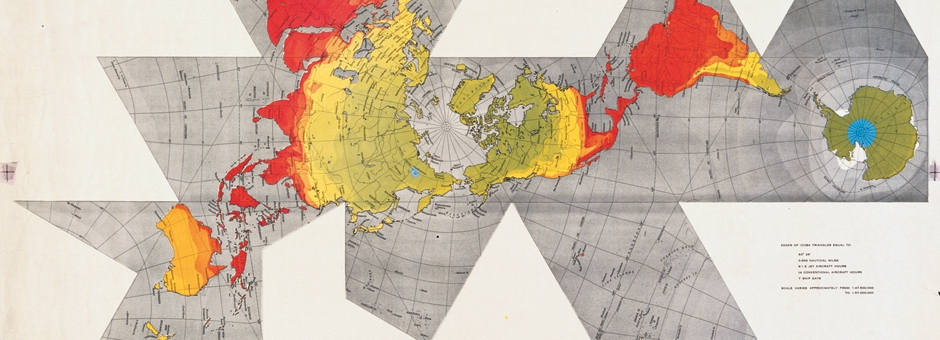
\includegraphics[width=0.9\textwidth]{2-2-dymaxmap}
        \end{center}
        
    \end{description}
    \end{solution}

    \question
    Describe how Phong's specular reflection models real specular reflection. Why is it only a rough approximation? Why is it useful?
    \begin{solution}
    Specular reflection is when the reflection of a light source is more intense at the angle of reflection (in contrast to diffuse reflection where the light is scattered in all directions).
    
    If $L_m$ is the direction of light from a light source $m$ then the direction of specular reflection $R$ is such that the normal to the surface bisects the angle subtended by the two directions.
    
    \begin{center}
        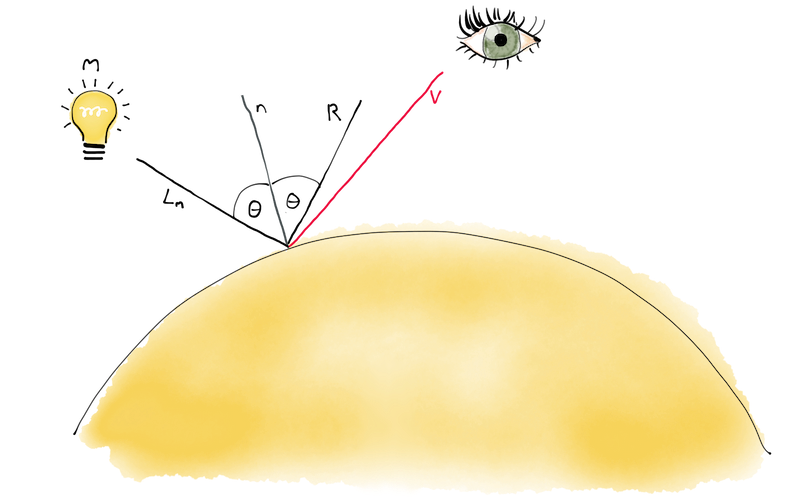
\includegraphics[width=0.9\textwidth]{2-3-specular}
    \end{center}
    
    For a perfect reflector then the reflection will only be visible in the direction $R$. For real objects (which are not perfect) the light can be seen even if the direction to the viewer $V$ does not coincide with $R$ (i.e. the reflection is visible within a cone around $R$). The shinier the surface the smaller this cone.
    
    Phong's model lets the intensity of the reflection by modelled by $cos(a)^n$, as this met the physical observation that for a shinier surface (larger $n$) the intensity drops off more rapidly.
    
    \begin{center}
        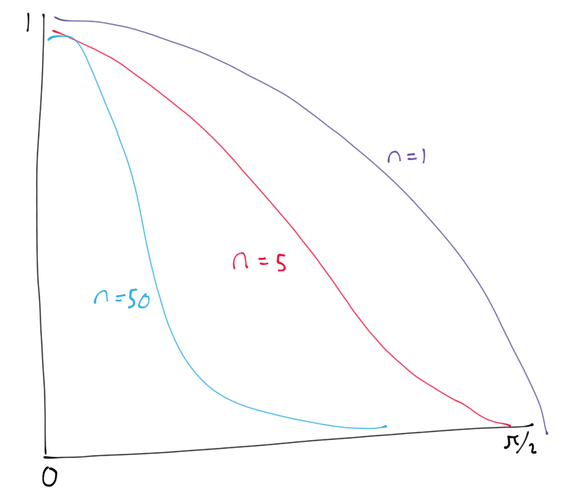
\includegraphics[width=0.5\textwidth]{2-3-phong}
    \end{center}
    
    Phong's model was based solely on physical observation rather than physics itself and the true rate at which the intensity falls off may not exactly match any power of $cos(a)$.
    
    True specular reflection is also a function of the incidence angle $\theta$. For example, glass reflects a lot more light when $\theta > 80\degree$). Some substances (e.g. copper) actually change colour with incidence angle.
    
    Phong approximates the \textit{reflectance distribution function} ($BRDF$) as the specular coefficient ($k_s$) and assumes it is constant (a reasonable approximation for many materials but not all).
    
    \end{solution}

    \question
    Draw pictures to show what is meant by:
    \begin{parts}
        \part{object coordinates}
        \part{world coordinates}
        \part{viewing coordinates}
        \part{screen coordinates}
    \end{parts}
    \begin{solution}
    \begin{center}
        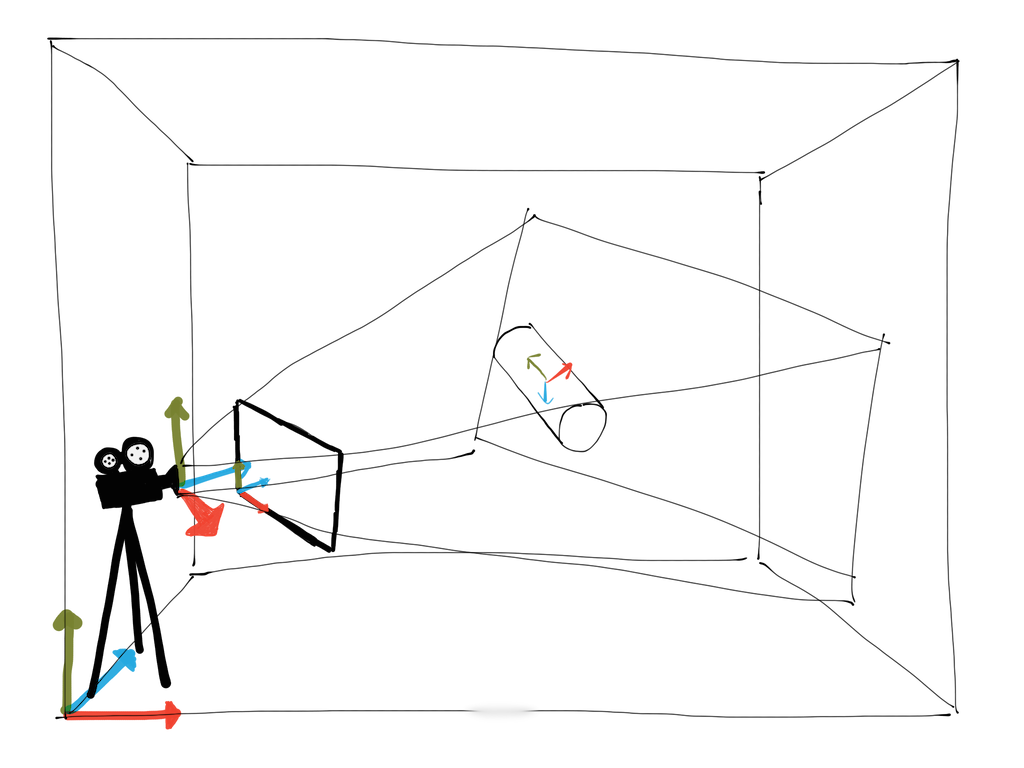
\includegraphics[width=0.8\textwidth]{2-4-coordinates}
    \end{center}
    \end{solution}

    \question
    We use a lot of triangles to approximate stuff in computer graphics. Why are they good? Why are they bad? Can you think of any alternatives?
    \begin{solution}
    Triangles are guaranteed to be planar which simplifies the maths involved with calculating normals. Any polygon can be split up into triangles.
    
    \textit{Not sure about disadvantages}
    
    Hexagons? 
    \end{solution}


\end{questions}

\section*{Longer Questions}
\begin{questions}
    \SetQuestionNumber{3}
    \question
    Draw and explain two different scenes which have the same projection as seen by the viewer. What other cues can you give so that the viewer can distinguish the depth information?
    \begin{solution}
    Focus can be used to show depth (make items in the background out of focus).
    \end{solution}

    \SetQuestionNumber{6}
    \question
    We often use triangles to represent a sphere. Describe two methods of generating triangles from a sphere.
    \begin{solution}
    \textit{Not sure about this}
    \end{solution}
    \question
    Compare and contrast:
    \begin{itemize}
        \item{texture mapping}
        \item{bump mapping}
        \item{displacement mapping}
    \end{itemize}
    \begin{solution}
    Texture mapping is where the surface of a \textit{3D} is mapped onto a \textit{2D} coordinate grid. A \textit{2D} texture can then be applied to the object.
    
    Bump mapping is a technique for simulating bumps or wrinkles on the surface of an object. A\textit{normal map} is mapped to the surface (in the same way a texture is mapped). This alters the normal at points on the surface and thus when the lighting is calculated it simulates bumps on the surface. It is useful when modelling an object that closely resembles a regular shape (e.g. a sphere) but has small disturbances on the surface. It is not suitable for large bumps as it doesn't alter the actual shape and thus at the edges of the sphere it will still be perfectly circular and thus will look strange. Also, since it only affects the normals it can't simulate self shadowing.
    
    Displacement mapping uses a map that actually changes the geometric position of points on the surface and thus in contrast to bump mapping it does allow for \textit{self-shadowing}.
    \begin{center}
        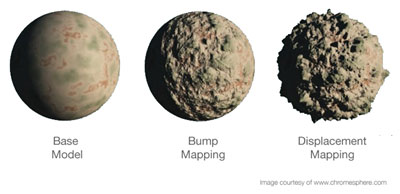
\includegraphics[width=0.8\textwidth]{2-7-mappings}
    \end{center}
    \end{solution}

    \SetQuestionNumber{10}
    \question
    \begin{parts}
        \part{Show how to perform 2D rotation around an arbitrary point.}
        \begin{solution}
        To rotate $\theta\degree$ about the origin you perform the following:
        \begin{center}
            $x'=x\cos{\theta}-y\sin{\theta}$ \\
            $y'=x\sin{\theta}+y\cos{\theta}$
        \end{center}
        To translate along vector $(t_x,t_y)$ you perform:
        \begin{center}
            $x'=x+t_x$ \\
            $y'=y+t_y$
        \end{center}
        
        A rotation about an arbitrary point is equivalent to a translation (such that the arbitrary point becomes the origin) then the rotation followed by the reverse translation.
        
        It is convenient (computationally) to represent these transformations as matrices as they can then be combined (using matrix multiplication). Since it is common to apply a transformation to several points it is often useful to be able to do some work once that is then used for every point.
        
        Since a translation transformation cannot be represented as a matrix when using a traditional coordinate representation we will use \textit{homogeneous coordinates}.
        
        The matrix for a rotation in homogeneous coordinates is:
        \begin{center}
            $
            \begin{pmatrix}
            \cos{\theta} & -\sin{\theta} & 0 \\ 
            \sin{\theta} &  \cos{\theta} & 0 \\ 
            0            & 0             & 1
            \end{pmatrix}
            $
        \end{center}
        
        The matrix for a translation in homogeneous coordinates is:
        
        \begin{center}
            $
            \begin{pmatrix}
            1 & 0 & t_x \\ 
            0 & 1 & t_y \\ 
            0 & 0 & 1
            \end{pmatrix}
            $
        \end{center}
        
        Thus, the transformation matrix representing a rotation of $\theta\degree$ about an arbitrary point $(p_x, p_y)$ is given by:
        
        \begin{center}
        
            $
            M =
            \begin{pmatrix}
            1 & 0 & -p_x \\ 
            0 & 1 & -p_y \\ 
            0 & 0 & 1
            \end{pmatrix}
            \times
            \begin{pmatrix}
            \cos{\theta} & -\sin{\theta} & 0 \\ 
            \sin{\theta} &  \cos{\theta} & 0 \\ 
            0            & 0             & 1
            \end{pmatrix}
            \times
            \begin{pmatrix}
            1 & 0 & -p_x \\ 
            0 & 1 & -p_y \\ 
            0 & 0 & 1
            \end{pmatrix}
            $
        \end{center}

 
        \end{solution}

        \part{Show how to perform 3D rotation around an arbitrary axis parallel to the \textit{x-axis}.}
        \begin{solution}
        The solution for a 3D rotation is largely the same as the 2D (just with an extra dimension). In the interest of brevity I will omit the steps and just show the final matrix calculation.
        
        \begin{center}
        $
            M =
            \begin{pmatrix}
            1 & 0 & 0 & 0 \\
            0 & 1 & 0 & -p_y \\
            0 & 0 & 1 & -p_z \\
            0 & 0 & 0 & 1
            \end{pmatrix}
            \times
            \begin{pmatrix}
            1 & 0 & 0 & 0\\
            0 & \cos{\theta} & -\sin{\theta} & 0 \\ 
            0 & \sin{\theta} &  \cos{\theta} & 0 \\ 
            0 & 0            & 0             & 1
            \end{pmatrix}
            \times
            \begin{pmatrix}
            1 & 0 & 0 & p_x \\
            0 & 1 & 0 & p_y \\
            0 & 0 & 1 & p_z \\
            0 & 0 & 0 & 1
            \end{pmatrix}
            $
        \end{center}

        \end{solution}

        \part{Show how to perform 3D rotation around an arbitrary axis.}
        \begin{solution}
        \textit{Not sure about this? I think it is a translation, 3 rotations (one around each orthogonal axis) followed by t but can't get it to work.}
        \end{solution}

    \end{parts}
    
\end{questions}

\section*{Advanced Questions}
\begin{questions}
    \SetQuestionNumber{3}
    \question
    Define and then compare and contrast the following methods of specifying rotation in 3D.
    
    \textit{You will need to look these up}.
    \begin{parts}
        \part{Quaternions}
        \begin{solution}
        The Quaternions $H$ are equal to $\mathbb{R}^4$, a four-dimensional vector space over the real numbers. $H$ has three operations:
        \begin{description}
            \item[Addition]
            Defined as their sum as elements of $\mathbb{R}^4$
            \item[Scalar multiplication]
            Defined as the product of each element by the scalar.
            \item[Quaternion multiplication]
            
            
        \end{description}
        \end{solution}

        \part{Euler Angles}

    \end{parts}
    \begin{solution}
    Euler angles do not interpolate in a consistent way and are thus less useful for animation where the interpolation matters (e.g. should animate smoothly between keyframes).
    
    Euler angles also suffer from \textit{Gimbal lock} (where a degree of freedom is lost when the axes of two of the gimbals are driven into a parallel configuration. This can be mitigated by altering the gimbal order but not completely avoided in some circumstances and requires additional thinking to get right.
    
    
    \end{solution}

    \question
    Find out about the Cook-Torrance shading model and explain how this improves on the naïve diffuse+specular+ambient model.
    \begin{solution}
    The \textit{Cook-Torrance} shading model models specular reflections using \textit{microfacets}. Essentially it models a surface as a "sea" of V-shaped facets that act like perfect mirrors. It takes into account the Fresnel effect (that materials become more \textit{specular} at glancing angles and are more \textit{Lambertian} towards normal incidence).
    
    This model allows for shadowing at the micro scale and thus more accurately represents the reflection intensity at large angles of incidence.
    \end{solution}


\end{questions}

\section*{Practical Programming}
\begin{questions}
    \question
    Write a program using OpenGL to display the scene that you rendered with your ray-tracer. Explore some different surface models in the fragment shader.
    \begin{solution}
    \begin{center}
        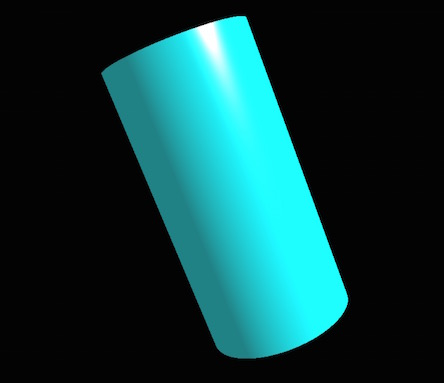
\includegraphics[width=0.5\textwidth]{2-p-screenshot}
    \end{center}
    Source can be seen at: \\
    \url{https://github.com/danielchatfield/cst1b-computer-graphics/}
    \end{solution}

\end{questions}


\end{document}
